\section{什么是数理统计?}

\begin{enumerate}
\item 统计学有一个别称——“数据科学”。
\item 统计学是一门研究不确定性的学科。
\item 统计学的本质是从不确定性中洞察确定性。
\item 参数估计和假设检验是统计学的根本任务。
\end{enumerate}

\section{概率论与数理统计的关联和差异}
统计学与数学分属两个学科,但是,绝多数人的认知仍是:统计是数学的一个分支。数学是一个古老的学科,而统计学是从数学中分化出来的,所以,时至今日,不少人仍有一个谬误:统计学是数学下的一个二级学科。学科的分化有一些典型的例子:计算机科学(CS)也是从数学中分化出来。而我们(数据学院)从当时计软学院独立出来的。

认识到统计学和数学是不同的学科后,同学们会有这样的一个困惑:概率论是数学的一个分支,数理统计是统计学的一个分支,那么为什么我们要把概率论与数理统计放在一起来上。这是因为统计是研究不确定性的学科,就目前而言,概率论是数学中对不确定性的一种科学测量,可能也是唯一的。就像马克思所说,“一门科学,只有当它成功地运用数学时,才能达到真正完善的地步。”在数理统计这部分中,我们需要使用到大量概率论的知识。同时,我们并未在任何先修课程中学过概率论的知识。于是,我们往往先了解概率论,再学习数理统计。

回顾一下在一个箱子里摸球的问题,如图\ref{fig:lect14_Prob&Stat1}。
概率论关注的是,已知这个箱子里有10个红球,有10个蓝球,从中随机抽出2个,求这2个球是什么情况?而数理统计关注的是,从装有20个球(部分是红球,部分是蓝球)的箱子里随机抽出2个球,已知这2个球分别是一红一蓝,求这20个球中有多少个红球,多少个蓝球?
\begin{figure}[ht]
    \centering
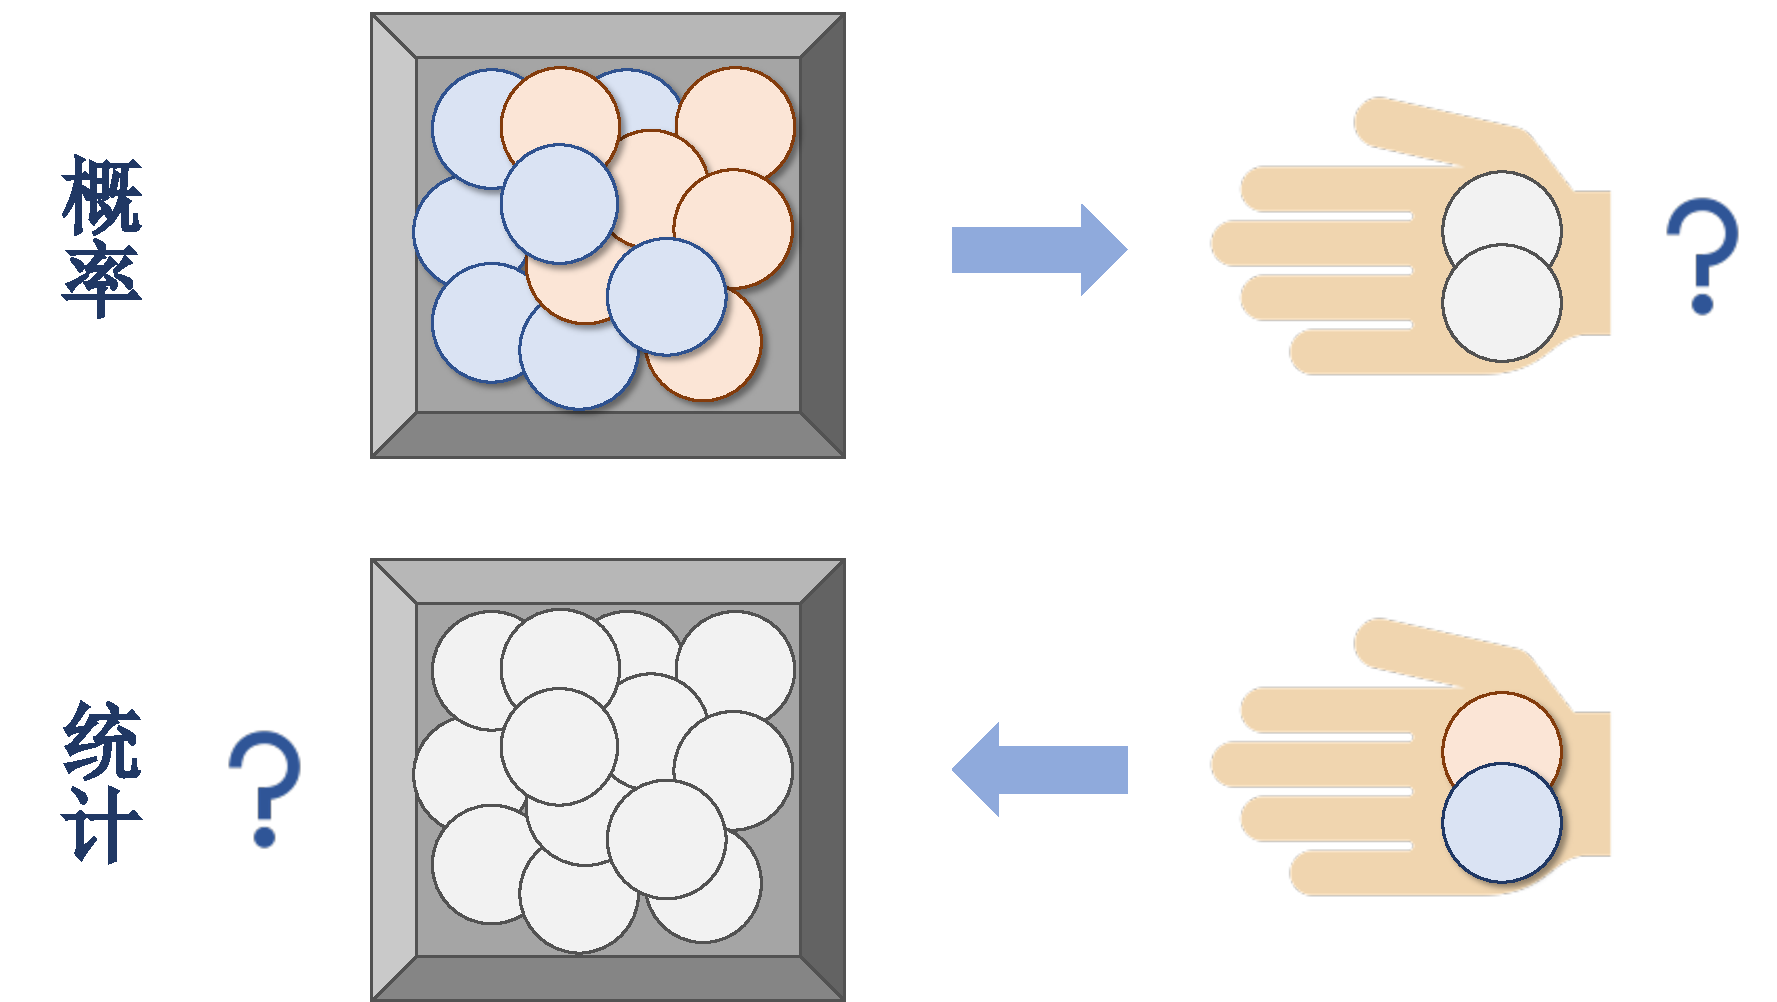
\includegraphics[scale=0.4]{image/Lectu14_Probability_and_Statistics.pdf}
\vspace{1cm}
    \caption{概率与统计的差别}
    \label{fig:lect14_Prob&Stat1}
\end{figure}

在上例中,我们从盒中取球,盒中的球我们称为“总体”,而取出的球为“样本”。在数理统计中,我们需要利用“样本”去\textbf{推断}“总体”。于是,有以下一些直观的理解:
\begin{enumerate}
    \item 合理的推断方法应该与样本的取值无关;(不能因人而异)
    \item 如果样本数量比较少,那么我们难以得到一个好的推断;(不能以蠡测海)
    \item 如果样本无法代表总体,那么我们无法得到一个好的推断;(不能盲人摸象)
\end{enumerate}

在数理统计中,我们所假定的总体是一个无穷总体。而样本的容量往往是有限的,记为$n$,表示样本量。基于上述的直观理解,样本被认为需要满足以下三个性质:
\begin{enumerate}
    \item 随机性;
    \item 可观测性;
    \item 可代表性;
\end{enumerate}
于是,我们将总体假定为一个随机变量$X$。所定义的样本$x_1,x_2,\cdots,x_n$,既可以表示随机变量$X_i$,也可以表示其取值$x_i$,这就是样本的两重性。而在数理统计这部分中,无特殊的情况说明,我们通常认为,样本与总体$X$是同一分布的,且样本是相互独立的随机变量,即
$$
x_1,x_2,\cdots,x_n\overset{\text{i.i.d}}{\sim} X.
$$
在本课程中,我们通过样本对总体进行推断,这与一般通过数据分析来进行预测任务的本质是相同的。因此,从这个意义上而言,数理统计是大家第一门数据分析类课程,或是数据分析类课程的先修课程。

\section{数理统计学点啥}
因为总体是一个随机变量,所以我们需要考虑其分布。
\begin{enumerate}
    \item 如果我们可以用有限个未知参数和固定的函数形式刻画这个分布,那么我们称这类模型假定为参数模型,常常记为$p(x;\bm{\theta}),\bm{\theta}\in \Theta$。这里是用密度来具体刻画,也可以写成分布函数的形式。例如,我们假定总体为正态分布,则均值$\mu$和方差$\sigma^2$就是未知参数。在频率学派中,我们认为未知参数是数,不具有随机性;而在贝叶斯学派中,我们认为未知参数是随机变量,具有随机性。
    \item 如果我们并未用未知参数来刻画这个分布,则称这个模型为非参数模型。
    \item 介于参数模型和非参数模型之间,有一类模型称为半参数模型,可以理解为这个分布表示方式中可以拆解为两个部分,一个部分是用参数模型刻画的,另一个部分是用非参数模型刻画的。
\end{enumerate}
\begin{remark}
    在非参数模型中,我们仍可以考虑其数字特征作为参数,例如:期望、方差、中位数等;
\end{remark}
在数理统计中,课内只学习参数模型$p(x;\bm{\theta})$。这是最简单的一个部分,也是非参数模型和半参数模型的基础。参数模型只是对总体分布的一种假定,我们核心任务可以划分为两类,估计和检验。
\begin{enumerate}
    \item 估计指的是,通过样本(数据)来得到未知参数$\bm{\theta}$的取值。在方法论层面,我们会学到有哪些估计的思想和相对应的方法,并我们会告诉大家如何比较两种估计方法的好坏。
    \item 检验指的是,通过样本(数据)来验证所猜想的假设$\bm{\theta}\in \Theta_0$是否成立。检验的思想是反证法——小概率事件不可能发生。我们会学到一些假设检验中的基本概念和框架,以及在正态总体分布假定下,单样本、二样本有关均值、方差的检验。
\end{enumerate}
